In 1996, David Sacket and colleagues defined \ac{ebm} as \textit{the conscientious, explicit, and judicious use of current best evidence in making decisions about the care of individual patients} \cite{sackettEvidenceBasedMedicine1996}. Despite having historical antecedents dating back to at least the 19th century, the first time the term "evidence-based medicine" was first coined by a team at McMaster University in Canada in the 1980s \cite{thomaBriefHistoryEvidenceBased2015}. This was a time when clinical decision-making was mostly based on untested observations and physicians' experience, leading to variability in treatment strategies. The birth of \ac{ebm} marked a pivotal moment in medical history, aiming to standardize patient care and improve outcomes. So, \ac{ebm} is still a relatively recent concept in healthcare, which entails integrating the best available research evidence with clinical experience and patient values to make decisions about patient care. 
With this, we can, as stated by Sacket, define \ac{ebm} into 3 major pillars:
\begin{myitemize}
    \item Best available evidence
    \item Clinical expertise
    \item Patient values, expectations, and/or wishes.
\end{myitemize}

Clinical expertise refers to the acumen and discernment gained from hands-on clinical experiences and consistent practice. This expertise manifests notably in enhanced diagnostic abilities and in the considerate recognition of a patient's unique circumstances, rights, and wishes when making care decisions. The term 'Best available evidence' pertains to pertinent clinical studies, often stemming from epidemiological investigations. This is linked with the ability (and willingness) to challenge current diagnostic methods and treatments, introducing alternatives that are more robust, precise, effective, and safer. 
Without experience, clinical practices blindly follow the best available evidence, which is not always the best option for the patient, since sometimes it may be inapplicable to a specific scenario. Without evidence, clinical practice becomes stagnated and unable to evolve \cite{sackettEvidenceBasedMedicine1996}.


The main concept of \ac{ebm} is the hierarchy of evidence, which classifies different types of research studies based on their methodological quality and applicability to patients. At the top of this hierarchy are \acp{rct} and systematic reviews of \acp{rct}, which are considered to provide the most robust evidence. Observational studies, case series, and expert opinions are further down the hierarchy due to their inherent limitations (figure \ref{fig:ebm}). \ac{ebm} advocates for the application of the highest level of evidence available in clinical decision-making.
\begin{figure}
    \centering
    %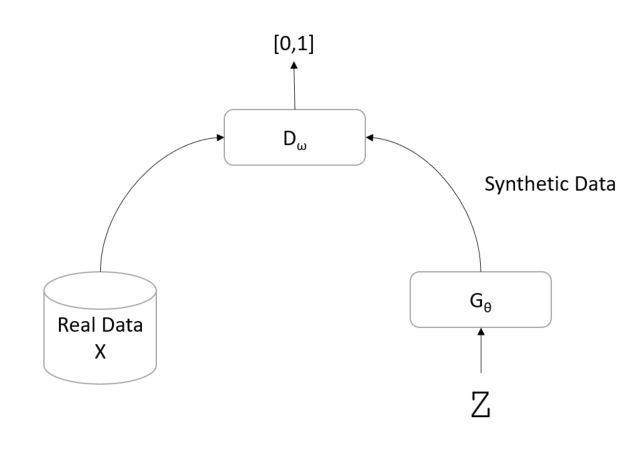
\includegraphics[width=\textwidth]{image.png}
    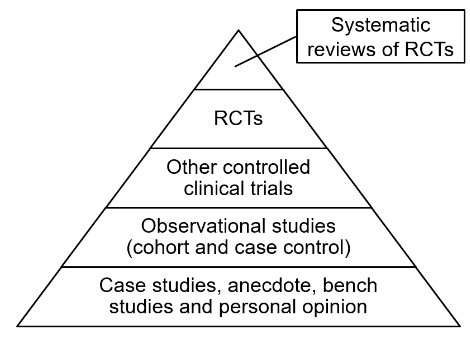
\includegraphics[scale=0.55]{figures/ebm.png}
    
    \caption{\ac{ebm}  adapted from \cite{greenhalghHowReadPaper2019}} \label{fig:ebm}
    \end{figure}

Historically, medical decisions leaned heavily on anecdotal observations and the prevailing beliefs of seasoned practitioners. To underscore the dangers of relying solely on such expert opinions, Sackett frequently recounted the circumstances surrounding George Washington's unfortunate end. Despite being in good health at the age of 68, Washington developed epiglottitis. Rather than opting for a tracheostomy, a treatment method known since ancient Greek times, his physicians, guided by the prevailing expert opinion, chose bloodletting as the course of action. Tragically, this decision led to Washington's likely preventable death, highlighting the critical importance of grounding medical decisions in robust evidence.
However, \ac{ebm} is not without critiques. The first one is that this is what medicine is all about and is already practiced all over. The data suggest something different \cite{sackettEvidenceBasedMedicine1996}.
The second refers to the virtually impossible task of keeping up with the literature. This argument, despite being refuted by examples of clinicians doing it, does raise the question of how we can deal with this, taking into account the increasing evidence overflow that the current times bring. How can we keep up with the literature and how can we make sure that the evidence is being applied in clinical practice? This is a very important question since the evidence is only useful if it is applied. This is where \ac{kdd} and \ac{ai} can play a role, as we will see in the next sections. 


